\documentclass[review]{elsarticle}

\usepackage{amsmath,amssymb,amsfonts}
\usepackage{algorithmic}
\usepackage{graphicx}
\usepackage{textcomp}
\usepackage{booktabs}
\usepackage{multirow}
\usepackage{hyperref}
\usepackage{xcolor}
\usepackage{subcaption}
\usepackage{siunitx}
\usepackage{lineno}

\journal{Ocean Engineering}

\begin{document}

\begin{frontmatter}

\title{WaveSplat: Grid-Free Spectral Wave Field Estimation\\from Sparse Shipboard LiDAR}

\author[avikus]{Saeyong Park\corref{cor1}}
\ead{saeyong.park@avikus.ai}
\cortext[cor1]{Corresponding author}
\address[avikus]{Avikus (HD Hyundai), Republic of Korea}

\begin{abstract}
We present WaveSplat, a grid-free method for real-time ocean wave field
estimation from sparse shipboard LiDAR observations.
Unlike grid-based approaches such as the Ensemble Transform Kalman Filter
(ETKF) that discretize the spatial domain and require interpolation of
sparse observations onto regular grids, WaveSplat represents the wave field
as a superposition of spectral components---plane waves parameterized
by wavenumber, amplitude, and phase---with angular frequency constrained by
the linear dispersion relation.
This continuous spectral representation avoids interpolation artifacts,
scales to arbitrary spatial resolution, and enables adaptive model
complexity matched to the true wave scene.

We propose a two-phase estimation pipeline: (1)~initialization via
dispersion-aware beamforming with coarse-to-fine refinement,
and (2)~per-frame tracking with physics-based phase prediction and selective
gradient updates.  A Fresnel-zone confidence weighting scheme accounts for
the range- and angle-dependent noise characteristics of LiDAR measurements
on ocean surfaces.

On 12 representative episodes spanning Beaufort~2--5 sea states
(1--30 wave components), WaveSplat achieves an average normalized RMSE
(nRMSE) of \textbf{0.211} compared to 0.436 for ETKF-grid
(\textbf{51.5\%} improvement), while running \textbf{2.4$\times$} faster
(13.4~vs.~31.7~ms/frame).
A multi-seed statistical validation (50 paired runs) confirms significance
($p < 0.001$, Wilcoxon signed-rank test).
The method is robust to both diffuse and specular LiDAR observation models,
winning on all 20 paired test episodes.
With adaptive model order, the method automatically selects $N$=1 for
simple swells and $N$=21 for complex multi-component seas,
achieving 6.4\% average improvement over fixed model order.
\end{abstract}

\begin{keyword}
wave field estimation \sep LiDAR \sep spectral methods \sep
dispersion relation \sep data assimilation \sep real-time estimation
\end{keyword}

\end{frontmatter}

\linenumbers

% ============================================================================
% Nomenclature
% ============================================================================
\begin{table}[h]
\centering
\caption{Nomenclature.}
\label{tab:nomenclature}
\begin{tabular}{ll}
\toprule
Symbol & Description \\
\midrule
$z(x,y,t)$ & Surface elevation [m] \\
$N$ & Number of spectral components \\
$w_i$ & Amplitude of $i$-th component [m] \\
$k_{x,i}, k_{y,i}$ & Wavenumber components [rad/m] \\
$\omega_i$ & Angular frequency [rad/s] \\
$\varphi_i$ & Phase offset [rad] \\
$g$ & Gravitational acceleration [m/s$^2$] \\
$d$ & Water depth [m] \\
$H_s$ & Significant wave height [m] \\
$T_p$ & Peak period [s] \\
$c_j$ & Confidence weight for observation $j$ \\
$\theta_j$ & Beam incidence angle [rad] \\
$M$ & Number of LiDAR observations per frame \\
nRMSE & RMSE normalized by $H_s$ \\
\bottomrule
\end{tabular}
\end{table}

% ============================================================================
\section{Introduction}
\label{sec:intro}

\subsection{Motivation: wave field information for maritime autonomy}

Knowledge of the ocean wave field surrounding a vessel is a prerequisite
for many functions in autonomous and semi-autonomous ship
operations~\citep{faltinsen2005, holthuijsen2007}.
Short-term wave prediction enables proactive motion compensation for
cargo handling and helicopter landing on offshore platforms~\citep{desmars2023}.
Route optimization algorithms require spatially resolved wave information
to minimize fuel consumption and structural fatigue
loading~\citep{vettor2016}.
Active ride control systems---particularly relevant for high-speed
hydrofoil vessels---can exploit wave preview for feedforward
disturbance rejection~\citep{park2026hydrofoil}.
Structural health monitoring benefits from accurate wave load estimation
for fatigue life assessment~\citep{DNV2010}.
In each application, the value of wave field information depends on
its spatial resolution, temporal update rate, and accuracy.

\subsection{Shipboard LiDAR for ocean surface sensing}

Several sensor modalities have been employed for sea surface observation.
Wave buoys provide accurate point measurements but lack spatial
resolution~\citep{datawell2009}.
X-band marine radar can image the sea surface over large areas
($\sim$2--4~km radius) but measures backscatter intensity rather than
elevation directly, requiring empirical or physics-based inversion to
recover wave spectra~\citep{nieto2004, young1985}.
Satellite altimetry provides global coverage at coarse spatial
resolution, unsuitable for real-time vessel-scale
applications~\citep{queffeulou2004}.

Shipboard scanning LiDAR has emerged as a compelling alternative,
providing \emph{direct} elevation measurements over a wide area at high
frame rates ($\sim$10~Hz)~\citep{nouguier2014, bjerkaas2022}.
Modern solid-state LiDAR systems (e.g., Seyond Falcon~K1: 1550~nm,
152~channels, $120^\circ \times 25^\circ$ FOV) can measure ocean
surface topography at ranges up to 250~m with centimeter-level
accuracy in the near field.
However, the observations are inherently sparse (typically 50--200 valid
surface returns per scan), unevenly distributed (denser near the ship
due to the fixed angular resolution), and noisy (accuracy degrades
with range due to beam divergence, and with incidence angle due to
specular reflection on the water surface).

The challenge is therefore to reconstruct a continuous, physically
consistent wave field from these sparse, heterogeneous observations
in real time.

\subsection{Grid-based paradigm and its limitations}

The dominant approach to this reconstruction problem follows a grid-based
data assimilation paradigm, adapted from numerical weather prediction:
discretize the spatial domain into a regular grid, represent the wave
state as surface elevation and velocity at grid points, and apply an
ensemble Kalman filter (EnKF/ETKF) to sequentially assimilate
observations~\citep{desmars2020, huhn2022, evensen2003}.
The ensemble forecast step propagates the wave state forward in time
using FFT-based spectral methods, which efficiently implement the
linear dispersion relation on regular grids.

While principled and well-studied, this grid-based approach has three
fundamental limitations when applied to sparse LiDAR observations:

\begin{enumerate}
  \item \textbf{Grid interpolation artifacts}: Sparse, irregularly
    distributed LiDAR observations must be mapped to grid
    points via interpolation or observation operators, introducing
    smoothing for wavelengths near the grid Nyquist limit and
    artificial correlations between neighboring grid cells.
    For a typical 40$\times$30 grid covering 200$\times$150~m,
    the grid spacing is 5~m, limiting the minimum resolvable
    wavelength to $\sim$10~m regardless of the LiDAR point density
    in the near field.
  \item \textbf{Fixed resolution}: The grid resolution is a design
    parameter that trades accuracy against computational cost.
    A fine grid ($80 \times 60$) improves resolution but
    quadruples the ensemble state dimension.
    Crucially, the grid resolution is fixed regardless of whether
    the actual wave field contains one or thirty spectral components,
    wasting computational resources on simple sea states and
    under-resolving complex ones.
  \item \textbf{Computational overhead}: The ensemble forecast requires
    FFT-based spectral propagation on the full grid for each of
    $N_e$ ensemble members, with cost scaling as
    $O(N_e \cdot G^2 \log G^2)$
    regardless of the true wave complexity.
    With typical values ($N_e = 50$, $G = 40 \times 30$), each
    forecast step involves 50 independent 2D FFTs.
\end{enumerate}

\subsection{Proposed approach}

We propose \textbf{WaveSplat}, a grid-free spectral representation
that eliminates the spatial grid entirely.
Instead of discretizing space, we represent the wave field as a weighted
superposition of $N$ plane waves:
\begin{equation}
  z(x, y, t) = \sum_{i=1}^{N} w_i \cos(k_{x,i} x + k_{y,i} y - \omega_i t + \varphi_i)
  \label{eq:forward}
\end{equation}
where each spectral component is parameterized by amplitude $w_i$,
wavenumber $(k_{x,i}, k_{y,i})$, and phase $\varphi_i$.
The angular frequency $\omega_i$ is not a free parameter but is
\emph{constrained} by the linear dispersion relation:
\begin{equation}
  \omega_i = \sqrt{g \, |k_i| \, \tanh(|k_i| \, d)}
  \label{eq:dispersion}
\end{equation}
where $g = 9.81$~m/s$^2$ and $d$ is the water depth.
This hard constraint reduces the parameter space from $5N$ to $4N$,
regularizes optimization, and ensures physically plausible wave
propagation during temporal tracking.

Our key contributions are:
\begin{enumerate}
  \item \textbf{Grid-free spectral estimation framework (C1)}: Direct
    estimation on sparse, irregularly distributed observations without
    grid interpolation, enabling continuous spatial evaluation at
    arbitrary resolution and naturally adapting to any observation
    pattern.
  \item \textbf{Dispersion-constrained parameterization (C2)}: Hard
    enforcement of the full dispersion relation (including $\tanh$
    depth dependence) reduces the free parameter count and acts as a
    physics-based regularizer, improving tracking stability over
    extended time horizons.
  \item \textbf{Fresnel-aware confidence weighting (C3)}: Per-observation
    weights based on incidence angle and range account for the
    heteroscedastic noise structure of LiDAR measurements on ocean
    surfaces, where specular reflection probability varies with
    local surface slope.
  \item \textbf{Adaptive model complexity}: Energy-based pruning and
    residual-triggered growth automatically match the number of spectral
    components to scene complexity, from $N$=1 for simple swells to
    $N$=21 for complex multi-component seas.
\end{enumerate}

The remainder of this paper is organized as follows.
Section~\ref{sec:related} reviews related work on wave field estimation.
Section~\ref{sec:method} presents the WaveSplat algorithm in detail.
Section~\ref{sec:experiments} describes the simulation environment and
evaluation metrics.
Section~\ref{sec:results} presents experimental results including
baseline comparisons, ablation studies, and robustness analysis.
Section~\ref{sec:discussion} discusses the findings and limitations.
Section~\ref{sec:conclusion} concludes.

% ============================================================================
\section{Related Work}
\label{sec:related}

We organize the review around two axes: (1)~the sensor modality
used for ocean surface observation, and (2)~the estimation algorithm
used to reconstruct the wave field from observations.
Table~\ref{tab:sensor_comparison} provides a quantitative comparison
of sensor modalities.

\begin{table*}[t]
\centering
\caption{Comparison of ocean surface sensing modalities for vessel-scale
wave field estimation. Typical values for operational systems.}
\label{tab:sensor_comparison}
\begin{tabular}{lccccl}
\toprule
Sensor & Spatial range & Resolution & Update rate & Direct elevation? & Key limitation \\
\midrule
Wave buoy & Point & --- & 1~Hz & Yes & No spatial information \\
X-band radar & 0.5--4~km & $\sim$7.5~m & 1--2~s/rev & No (intensity) & Requires SNR inversion \\
Satellite (altimeter) & Global & $\sim$7~km & Days & Yes (nadir) & Coarse, non-real-time \\
Shipboard LiDAR & 10--250~m & $\sim$0.1~m (near) & 10~Hz & Yes & Sparse, range-dependent noise \\
Ship motion (RAO) & --- & --- & Continuous & No (indirect) & Limited to encountered waves \\
\bottomrule
\end{tabular}
\end{table*}

\subsection{X-band radar-based wave estimation}

X-band marine radar has been the most extensively studied sensor for
shipboard wave field estimation.
\citet{young1985} first demonstrated that the modulation of radar
backscatter by ocean waves (through tilt modulation, hydrodynamic
modulation, and shadowing) carries extractable wave spectral
information.
\citet{nieto2004} developed a comprehensive inversion algorithm that
recovers the directional wave spectrum from radar image sequences
using 3D FFT in the $(k_x, k_y, \omega)$ domain, with the linear
dispersion relation serving as a spectral filter to separate wave
signals from noise.
This ``dispersion filtering'' concept---using the known relationship
between wavenumber and frequency to constrain spectral
estimation---is conceptually related to our dispersion-constrained
parameterization, though applied in the Fourier domain rather than
as a hard parameter constraint.

A fundamental limitation of radar-based methods is that radar
measures backscatter intensity rather than surface elevation directly.
The intensity-to-elevation mapping requires an empirical modulation
transfer function (MTF) that depends on radar parameters, wind speed,
and sea state~\citep{nieto2004}.
Additionally, the spatial resolution of X-band radar ($\sim$7.5~m for
typical 9~GHz systems) is coarser than LiDAR ($\sim$0.1~m in the near
field), limiting the resolvable wavelength range.

\subsection{Ship-motion-based wave estimation}

An alternative approach estimates the wave field indirectly from
measured vessel motions.
\citet{naaijen2018} and \citet{nielsen2006} developed methods that
invert the ship's response amplitude operator (RAO) to recover the
incident wave spectrum from measured heave, pitch, and roll motions.
These methods require no additional sensors beyond standard IMU/GPS
but are limited to the frequency range where the vessel has
measurable response, and they cannot resolve the spatial wave field---only
the directional spectrum at the vessel's location.
WaveSplat provides complementary information: a spatially resolved
wave field in the LiDAR observation area, enabling applications such
as spatial wave preview for feedforward control.

\subsection{Grid-based wave field reconstruction}

Deterministic wave field reconstruction from spatially resolved
sensor data has been an active research area since the 2010s.
The dominant paradigm combines spatial discretization with ensemble
data assimilation.
\citet{desmars2020} introduced ETKF-based wave field reconstruction from
X-band radar, using spectral propagation on a regular spatial grid as the
forecast model.  The Ensemble Transform Kalman Filter~\citep{hunt2007}
is favored over the stochastic EnKF~\citep{evensen2003} for its
deterministic analysis step and better preservation of the ensemble mean.
\citet{huhn2022} extended this framework to LiDAR observations,
demonstrating the ``from points to waves'' pipeline on both fixed-platform
and shipboard data, with grid resolutions of 40$\times$30 to 80$\times$60.
\citet{desmars2023} demonstrated real-time reconstruction and
short-term deterministic prediction up to one peak period ahead,
with prediction skill degrading beyond the theoretical
predictability horizon determined by the group velocity of the
shortest resolved component.

It is important to distinguish \emph{deterministic} reconstruction
(recovering the instantaneous wave field phase) from
\emph{stochastic} wave prediction (forecasting statistical properties
such as significant wave height or spectral density).
WaveSplat and the ETKF methods above perform deterministic
reconstruction: they estimate the phase of each wave component,
enabling spatial evaluation at arbitrary points.
Stochastic methods---including spectral wave models like
WAVEWATCH~III~\citep{tolman2009}---predict the evolution of the
wave energy spectrum without resolving individual phases and
operate at much coarser spatial scales (kilometers to tens of
kilometers).

These grid-based deterministic methods share a common architecture:
discretize the 2D spatial domain into a regular grid, maintain an
ensemble of spectral states, and assimilate observations via the
Kalman update.
The grid discretization introduces an inherent trade-off between
spatial resolution and computational cost, and the interpolation from
sparse observations to grid points is a known source of error,
particularly for wavelengths near the grid Nyquist limit.

\subsection{Spectral estimation from irregular arrays}

Classical spectral estimation methods (FFT, Welch, MUSIC, ESPRIT) assume
regularly sampled data and cannot directly handle the irregular, sparse
sampling inherent to scanning LiDAR~\citep{young1994}.
Capon's minimum-variance beamforming~\citep{capon1969} can accommodate
irregular sensor arrays but assumes signal stationarity and provides
only a power spectral density estimate without individual component
phases.
The MUSIC algorithm~\citep{schmidt1986} can super-resolve closely
spaced spectral peaks from short data records but requires knowledge
of the number of sources and is sensitive to model order
misspecification.
Iterative adaptive approaches (IAA) extend Capon to non-stationary
scenarios but remain computationally expensive for high-resolution
wavenumber grids ($O(N_k^2 \cdot M)$ per iteration, where $N_k$ is
the number of wavenumber grid points).

WaveSplat leverages beamforming for initialization---extracting
dominant wavenumber peaks from irregular LiDAR
observations---but then refines these estimates through gradient-based
optimization that jointly recovers amplitudes and phases, exploiting
temporal structure through the dispersion relation.
This two-stage approach combines the robustness of beamforming
(no local minima in wavenumber space) with the precision of
optimization (joint amplitude-phase recovery with physics constraints).

\subsection{Gaussian process regression for wave fields}

Gaussian process regression (GPR) offers a nonparametric alternative
for spatial interpolation of wave fields from scattered
observations~\citep{rasmussen2006}.
With a Mat\'{e}rn or squared-exponential kernel, GPR can capture the
spatial correlation structure of ocean waves without assuming a specific
spectral model, and the posterior variance provides natural uncertainty
quantification.

However, GPR has fundamental limitations for real-time wave estimation.
The standard formulation requires $O(M^3)$ computation and $O(M^2)$
storage for $M$ observations, making it impractical at high observation
densities.
Sparse GPR approximations using inducing points~\citep{titsias2009}
reduce the cost to $O(M \cdot P^2)$ for $P \ll M$ inducing points,
but the inducing point placement and kernel hyperparameter optimization
add complexity.
More fundamentally, standard GPR operates on single frames without a
temporal propagation model, losing the physics of wave evolution.
Incorporating temporal dynamics into a GPR framework (e.g., via
spatio-temporal kernels encoding the dispersion relation) is an active
research area but has not been demonstrated for real-time applications.

\subsection{Neural and learning-based approaches}

Recent work has applied deep learning to ocean wave
prediction~\citep{zhang2022, mohaghegh2021}, including physics-informed
neural networks (PINNs) that incorporate wave equations as soft
constraints in the loss function.
\citet{zhang2022} demonstrated that PINNs can improve generalization
for wave prediction by penalizing violations of the linear wave
equation, though the approach requires retraining for each sea state
configuration.
Encoder-decoder architectures have also been applied to reconstruct
spatial wave fields from sparse measurements, achieving promising
results in offline settings~\citep{mohaghegh2021}.

While these methods are promising for offline analysis, they face
practical challenges for real-time shipboard deployment:
(1)~training data requirements---collecting sufficient paired
(sparse observation, dense ground truth) datasets for diverse sea
states is expensive;
(2)~generalization---models trained on one sensor configuration or
sea state may not transfer well;
(3)~interpretability---the black-box nature of neural networks makes
it difficult to diagnose failure modes or ensure physical
consistency (e.g., correct dispersion behavior).
WaveSplat requires no training data and produces directly interpretable
spectral parameters (wavenumber, amplitude, frequency, phase) that
satisfy the dispersion relation by construction.

\subsection{Sparse and adaptive signal representations}

The idea of representing physical fields as weighted sums of
basis functions with adaptive complexity has a long history in
signal processing and computational physics.
Compressed sensing theory~\citep{candes2006} establishes that sparse
signals can be exactly recovered from far fewer measurements than
the Nyquist limit, provided the measurement matrix satisfies a
restricted isometry property.
Matching pursuit algorithms~\citep{mallat1993} provide greedy
approximations by iteratively selecting basis functions from
overcomplete dictionaries.
In the oceanographic context, \citet{drazen2008} applied sparse
spectral representations to reconstruct wave fields from pressure
sensors, demonstrating that the wave field's inherent spectral
sparsity enables efficient reconstruction.

WaveSplat extends this philosophy with two key differences:
(1)~each basis function is a physically meaningful plane wave
satisfying the dispersion relation, rather than a generic sinusoid
or wavelet; and
(2)~the model order is adapted \emph{online} (during tracking) based
on residual energy and observation quality, rather than being fixed
a priori.

% ============================================================================
\section{Method}
\label{sec:method}

\subsection{Forward model}

The wave field is modeled as a superposition of $N$ linear plane
waves~\eqref{eq:forward}.
Each component $i$ has four free parameters: amplitude $w_i$,
wavenumber components $(k_{x,i}, k_{y,i})$, and phase offset
$\varphi_i$. The angular frequency $\omega_i$ is deterministically
computed from the dispersion relation~\eqref{eq:dispersion},
reducing the total parameter count from $5N$ to $4N$.

This linear forward model is an $O(\epsilon^2)$ approximation to
higher-order wave theories (e.g., Gerstner waves or second-order
Stokes), where $\epsilon = |k| \cdot |w|$ is the wave steepness.
At Beaufort~4, typical steepness is $\epsilon \approx 0.05$,
giving a model mismatch of $< 0.25\%$.
For the Beaufort~2--5 range considered in this work
(non-breaking waves), the linear model is an excellent
approximation~\citep{holthuijsen2007}.

\subsection{Observation model}

At each LiDAR scan at time $t$, we observe $M$ elevation measurements
$\{(x_j, y_j, z_j)\}_{j=1}^{M}$ at irregular spatial locations.
The observation model is:
\begin{equation}
  z_j = \sum_{i=1}^{N} w_i \cos(k_{x,i} x_j + k_{y,i} y_j - \omega_i t + \varphi_i) + \eta_j
\end{equation}
where $\eta_j$ is observation noise with variance depending on range
and incidence angle.  The number of valid observations per frame
varies between 50 and 200, depending on sea state, vessel motion,
and LiDAR raydrop characteristics.

\subsection{Fresnel-zone confidence weighting (C3)}

LiDAR elevation accuracy on ocean surfaces degrades with two
physical mechanisms:
(1)~beam divergence increases the footprint area at longer ranges,
averaging over local surface curvature; and
(2)~at high incidence angles (near-grazing geometry), the probability
of specular reflection increases, causing either total signal loss
or biased returns from wave crests.

We assign per-observation confidence weights:
\begin{equation}
  c_j = \frac{\cos(\theta_j)}{d_j / d_{\text{ref}}}
  \label{eq:confidence}
\end{equation}
where $\theta_j$ is the beam incidence angle (computed from the
local surface normal and beam direction), $d_j$ is the range,
and $d_{\text{ref}} = 125$~m is a reference distance chosen as
half the maximum LiDAR range.
These weights are incorporated in the optimization loss as weighted
mean squared error, giving higher influence to close-range,
near-normal observations.

\subsection{Two-phase estimation}

The estimation proceeds in two phases: an initialization phase that
establishes the spectral model from multi-frame observations, followed
by a per-frame tracking phase that maintains the model with
minimal computation.  Algorithm~\ref{alg:wavesplat} summarizes
the complete pipeline.

\begin{table}[t]
\centering
\caption{Algorithm: WaveSplat estimation pipeline.}
\label{alg:wavesplat}
\begin{tabular}{p{0.92\columnwidth}}
\toprule
\textbf{Phase 1: Initialization} (frames $1$ to $T_\text{init}/\Delta t$) \\
\midrule
1. Accumulate multi-frame observations $\{(x_j, y_j, z_j, t_j)\}$ \\
2. Compute beamforming power $P(k_x, k_y)$ on polar grid \\
3. Extract top-$N$ wavenumber peaks with greedy suppression \\
4. Estimate amplitudes/phases via linear least-squares \\
5. Coarse-to-fine refinement: $N$=3 $\to$ 8 $\to$ 15 \\
\quad --- At each stage: 200 Adam steps, lr=$5\times 10^{-3}$ \\
6. Energy-based pruning (retain 90\% energy) \\
7. Safety check: if $\Delta\text{RMSE} > 30\%$, rollback \\
8. Residual growth: if RMSE $> 0.05$~m, add via beamforming \\
\midrule
\textbf{Phase 2: Tracking} (each subsequent frame) \\
\midrule
1. \textbf{Predict}: $\varphi_i \mathrel{+}= \omega_i \cdot \Delta t$ \\
2. \textbf{Update}: $K$=10 Adam steps on sliding window ($K_w$=3 frames) \\
\quad --- Update only $(w_i, \varphi_i)$; freeze $(k_{x,i}, k_{y,i})$ \\
\quad --- Learning rate: $1\times 10^{-3}$, no scheduling \\
\bottomrule
\end{tabular}
\end{table}

\subsubsection{Phase 1: Initialization}

Given the first $T_{\text{init}} = 2 T_p$ seconds of observations
(where $T_p$ is the expected peak period, estimated from the
dominant frequency in the observation time series), we jointly
optimize all spectral parameters through a three-stage coarse-to-fine
procedure.

\textbf{Dispersion-aware beamforming.}
Initial wavenumber estimates are obtained by scanning a polar grid
in wavenumber space.  The grid covers
$|k| \in [0.02, 0.50]$~rad/m (corresponding to wavelengths
$\lambda = 2\pi/|k| \in [12.6, 314]$~m, spanning Beaufort~2--5
conditions at $d$=50~m depth) with 64~radial $\times$ 128~azimuthal
bins.  The radial range is determined by the dispersion relation:
$|k|_\text{min} = 0.02$ corresponds to BF5 swell ($T_p \approx 9$~s),
and $|k|_\text{max} = 0.50$ corresponds to the shortest wavelength
resolvable from the LiDAR spatial extent ($\sim$200~m observation
radius).

For each candidate $(k_x, k_y)$, we compute
$\omega = \sqrt{g|k|\tanh(|k|d)}$ and evaluate the beamforming power:
\begin{equation}
  P(k_x, k_y) = \left| \sum_{j} z_j \, e^{-i(k_x x_j + k_y y_j - \omega t_j)} \right|^2
\end{equation}
where the summation runs over all observations accumulated during
$T_\text{init}$.  The use of the dispersion-derived $\omega$ means
that the beamforming naturally filters for physically plausible
wave signals, suppressing noise that does not lie on the
dispersion surface in $(k_x, k_y, \omega)$ space.

Peaks in $P$ are extracted greedily: the maximum is selected, then
all candidates within $15^\circ$ angular separation are suppressed,
and the process repeats.  The $15^\circ$ threshold prevents double-
counting of the same wave component spread across adjacent
wavenumber bins, while being narrow enough to resolve crossing sea
systems.  The initial amplitude and phase of each extracted component
are estimated via linear least-squares projection of the accumulated
observations onto the selected wavenumber basis functions.

\textbf{Coarse-to-fine optimization.}
Starting from the beamforming initialization, we optimize the
spectral parameters in three stages ($N$=3 $\to$ 8 $\to$ 15),
with 200 iterations of the Adam optimizer~\citep{kingma2015}
(learning rate $\eta = 5 \times 10^{-3}$,
$\beta_1 = 0.9$, $\beta_2 = 0.999$) at each stage.
The loss function is:
\begin{equation}
  \mathcal{L} = \underbrace{\frac{1}{M} \sum_j c_j \, (z_j - \hat{z}_j)^2}_{\text{weighted MSE}}
    + \underbrace{\lambda_1 \sum_i |w_i|}_{\text{sparsity}}
    + \underbrace{\lambda_s \sum_i (w_{\sigma(i)} - w_{\sigma(i-1)})^2}_{\text{spectral smoothness}}
\end{equation}
where $\lambda_1 = 10^{-3}$ promotes amplitude sparsity (driving
negligible components toward zero for subsequent pruning) and
$\lambda_s = 10^{-4}$ penalizes abrupt amplitude variations between
spectrally adjacent components ($\sigma$ denotes ordering by $|k|$),
encouraging smooth spectral envelopes consistent with JONSWAP-like
spectra.

During optimization, wavenumber components $(k_{x,i}, k_{y,i})$
are free parameters (unlike in the tracking phase).  The dispersion
constraint is enforced by computing $\omega_i$ from $(k_{x,i}, k_{y,i})$
at each forward evaluation rather than treating $\omega_i$ as a free
parameter, ensuring that the constraint is satisfied exactly
throughout optimization.

\subsubsection{Adaptive model order}

After initialization, we apply energy-based pruning.
Components are sorted by energy $E_i = w_i^2$ in descending order,
and the minimum set capturing 90\% of total energy
$\sum_i E_i$ is retained.  This criterion is motivated by the
JONSWAP spectral shape, where a small number of components near the
spectral peak typically contain the majority of the wave energy.

A safety check prevents aggressive pruning from discarding physically
significant components: if the post-pruning RMSE exceeds
130\% of the pre-pruning value, pruning is rolled back entirely.
This can occur when two components of similar energy
contribute to different spatial regions (e.g., crossing seas),
making each individually appear low-energy.

If the residual RMS after pruning exceeds 0.05~m (indicating
unmodeled wave energy), new components are grown by applying
beamforming to the residual signal $r_j = z_j - \hat{z}_j$ and
adding the dominant residual peaks to the model, up to
$N_{\max}=30$.

\subsubsection{Phase 2: Tracking}

For each subsequent LiDAR frame, we perform a predict--update cycle:
\begin{enumerate}
  \item \textbf{Predict}: advance phases using the dispersion-derived
    angular frequency, $\varphi_i \mathrel{+}= \omega_i \, \Delta t$,
    where $\Delta t = 0.1$~s (10~Hz LiDAR frame rate).
    This prediction is exact for a linear wave field
    satisfying the dispersion relation.
  \item \textbf{Update}: perform $K=10$ Adam steps
    (lr$=1\times 10^{-3}$) on the weighted MSE loss over a
    sliding window of $K_w=3$ recent frames, updating only
    amplitudes $w_i$ and phases $\varphi_i$ while freezing
    wavenumbers $(k_{x,i}, k_{y,i})$ (\texttt{w\_phi} tracking mode).
\end{enumerate}

Freezing wavenumbers during tracking is motivated by two considerations:
(1)~wavenumber estimation from a single frame is ill-conditioned due
to spatial aliasing in sparse observations---the LiDAR's irregular
sampling pattern does not provide sufficient constraint to resolve
wavenumber from a single snapshot, while the multi-frame
initialization averages over $\sim$20 frames to obtain robust
wavenumber estimates; and
(2)~with fixed wavenumbers, the dispersion constraint provides a
strong phase prediction ($\omega \cdot \Delta t$) that serves as a
warm start, reducing the gradient steps needed per frame from
$\sim$200 (full optimization) to 10.

The sliding window ($K_w = 3$) uses the three most recent frames
for gradient computation.  This provides temporal averaging that
smooths single-frame noise without introducing excessive latency:
at 10~Hz, the window spans 0.3~s, much shorter than the peak
period $T_p$ for all sea states considered.

\subsection{Computational complexity}

Let $M$ denote the number of LiDAR observations per frame and
$N$ the number of spectral components.

\textbf{WaveSplat}: Each forward evaluation computes
$z(x_j, y_j, t) = \sum_{i=1}^{N} w_i \cos(\cdot)$,
costing $O(M \cdot N)$ per frame. With $K$ gradient steps and window
size $K_w$, the per-frame tracking cost is $O(K \cdot K_w \cdot M \cdot N)$.
In practice, $K{=}10$, $K_w{=}3$, $N \leq 30$, yielding 13.4~ms/frame
on CPU (single-threaded, Intel i7-12700H).

\textbf{ETKF-grid}: The Ensemble Transform Kalman Filter maintains
$N_e$ ensemble members on a $G_x \times G_y$ spatial grid.
Each update involves FFT-based propagation at
$O(N_e \cdot G_x G_y \cdot \log(G_x G_y))$ plus the ensemble
transform at $O(N_e^3 + N_e^2 \cdot M)$. With $N_e{=}50$ and
$G{=}40 \times 30$, this yields 31.7~ms/frame.

\textbf{GPR}: Gaussian Process Regression with $M$ observations
requires $O(M^3)$ for Cholesky factorization, making it impractical
for dense LiDAR data. Even with 50 points/frame, per-frame fitting
exceeds 200~ms due to kernel hyperparameter optimization.

Table~\ref{tab:complexity} summarizes the scaling comparison.

\begin{table}[t]
\centering
\caption{Computational complexity comparison.
$M$: observations/frame, $N$: spectral components,
$G$: grid size, $N_e$: ensemble members.}
\label{tab:complexity}
\begin{tabular}{lcc}
\toprule
Method & Per-frame complexity & Measured \\
\midrule
WaveSplat & $O(K \cdot K_w \cdot M \cdot N)$ & 13.4~ms \\
ETKF-grid & $O(N_e \cdot G^2 \log G^2)$ & 31.7~ms \\
GPR       & $O(M^3)$ & $>$200~ms \\
\bottomrule
\end{tabular}
\end{table}

% ============================================================================
\section{Experimental Setup}
\label{sec:experiments}

\subsection{Simulation environment}

We develop a physics-based LiDAR wave simulation (WaveSim) generating
ground-truth wave fields with JONSWAP spectrum
sampling~\citep{hasselmann1973}.  The simulator parameters are:
\begin{itemize}
  \item \textbf{Sea states}: Beaufort~2--5
    ($H_s$=0.3--2.0~m, $T_p$=4--9~s)
  \item \textbf{Wave complexity}: 1, 2, 5, 15, 30 spectral components
    with directional spreading ($\pm 20^\circ$)
  \item \textbf{Ground-truth wave model}: Gerstner waves (nonlinear),
    providing a realistic test of the linear forward
    model~\eqref{eq:forward}
  \item \textbf{LiDAR model}: 500 horizontal beams, 10~Hz scan rate,
    range 10--250~m, based on the Seyond Falcon~K1 specifications
    (1550~nm, 152~channels, $120^\circ \times 25^\circ$ FOV)
  \item \textbf{Raydrop models}: (a)~uniform---constant drop probability
    independent of surface geometry (diffuse Fresnel reflection); and
    (b)~slope-dependent---higher dropout on steep surfaces with
    near-grazing geometry (specular backscatter model)
  \item \textbf{Water depth}: $d = 50$~m (intermediate to deep water
    for the wavelengths considered)
\end{itemize}

Each episode contains 301 frames (30~s at 10~Hz) with ground-truth
elevation fields evaluated on a 80$\times$60 spatial grid
covering the LiDAR observation area.
A total of 100 episodes are generated across 5 random seeds per
configuration, from which 12 representative episodes are selected
for the main comparison (covering all Beaufort numbers and complexity
levels) and 50 paired runs are used for statistical validation.

\subsection{Metrics}

We report:
\begin{itemize}
  \item \textbf{nRMSE}: RMSE normalized by significant wave height $H_s$,
    the primary reconstruction quality metric.
    Lower is better; values below 0.10 indicate excellent reconstruction,
    0.10--0.30 is good, and above 0.30 indicates significant error.
  \item \textbf{Inference speed}: ms/frame for the tracking phase,
    measured on a single CPU thread.
  \item \textbf{$N_{\text{adapt}}$}: final number of spectral components
    after adaptive model order selection.
\end{itemize}

\subsection{Baselines}

\textbf{ETKF-grid}~\citep{huhn2022}: Ensemble Transform Kalman Filter
on a 40$\times$30 regular grid with 50 ensemble members,
FFT-based spectral propagation, multiplicative ($\alpha$=1.01) and
additive ($\sigma$=0.005) inflation, and observation thinning to
$M_{\max}$=40 per frame.  This configuration follows the
recommendations of \citet{huhn2022} for shipboard LiDAR scenarios.

\textbf{GPR}: Gaussian Process Regression with Mat\'{e}rn $\nu$=5/2
kernel (length scale 20~m, noise $\sigma$=0.02~m), operating in
single-frame mode.
No temporal model or physics constraints---pure spatial interpolation.
This represents the best achievable single-frame performance without
wave physics, providing a reference for the value of temporal tracking
and dispersion constraints.

% ============================================================================
\section{Results}
\label{sec:results}

\subsection{Main comparison}

Table~\ref{tab:main} summarizes the comparison across 12 representative
episodes. WaveSplat achieves an average nRMSE of \textbf{0.211} compared
to 0.436 for ETKF-grid, a \textbf{51.5\%} improvement.
WaveSplat wins on all 12 episodes.

We additionally compare with GPR on 10 uniform-raydrop episodes.
GPR achieves avg nRMSE of 0.276---better than ETKF (0.450) due to
its nonparametric flexibility, but still 23.5\% worse than WaveSplat
(0.233). Critically, GPR requires $>$200~ms/frame (vs.\ 13.4~ms for
WaveSplat), making it impractical for real-time applications.
Figure~\ref{fig:qualitative} shows representative wave fields.

\begin{table}[t]
\centering
\caption{WaveSplat vs ETKF-grid on 12 representative episodes.
nRMSE = RMSE/$H_s$; lower is better. $N_a$ = adapted component count.}
\label{tab:main}
\begin{tabular}{lccccc}
\toprule
& \multicolumn{2}{c}{WaveSplat} & \multicolumn{2}{c}{ETKF} & \\
\cmidrule(lr){2-3} \cmidrule(lr){4-5}
Episode & nRMSE & ms/f & nRMSE & ms/f & $N_a$ \\
\midrule
BF2 1comp     & \textbf{0.315} & 13.8 & 0.483 & 29.1 & 11 \\
BF3 1comp     & \textbf{0.217} & 13.0 & 0.352 & 36.8 &  2 \\
BF3 2comp (U) & \textbf{0.052} & 15.0 & 0.444 & 37.2 &  2 \\
BF3 2comp (S) & \textbf{0.061} & 13.4 & 0.350 & 26.3 & 15 \\
BF3 5comp (U) & \textbf{0.167} & 13.0 & 0.434 & 29.6 &  4 \\
BF3 5comp (S) & \textbf{0.152} & 13.4 & 0.384 & 32.7 & 15 \\
BF4 1comp     & \textbf{0.171} & 11.2 & 0.410 & 26.7 &  1 \\
BF4 5comp     & \textbf{0.200} & 12.8 & 0.376 & 28.7 &  3 \\
BF4 15comp    & \textbf{0.302} & 13.4 & 0.511 & 25.8 & 19 \\
BF4 30comp    & \textbf{0.314} & 13.4 & 0.525 & 28.3 & 18 \\
BF5 15comp    & \textbf{0.297} & 13.5 & 0.466 & 27.2 & 21 \\
BF5 30comp    & \textbf{0.290} & 14.7 & 0.497 & 52.2 & 19 \\
\midrule
\textbf{Avg}  & \textbf{0.211} & 13.4 & 0.436 & 31.7 & --- \\
\bottomrule
\end{tabular}
\end{table}

Key observations:
\begin{itemize}
  \item \textbf{Low complexity}: For BF3 2-component seas, WaveSplat
    achieves nRMSE=0.052, an 8.5$\times$ advantage over ETKF (0.444).
    The grid-free representation directly captures two plane waves
    without grid aliasing.
  \item \textbf{High complexity}: For BF4--5 with 15--30 components,
    WaveSplat still outperforms ETKF (0.301 vs.\ 0.500 average),
    though the gap narrows as the spectral complexity approaches the
    initialization resolution limit.
  \item \textbf{Speed}: WaveSplat runs at 13.4~ms/frame
    vs.\ 31.7~ms for ETKF (2.4$\times$ faster), well within the
    100~ms real-time budget for 10~Hz LiDAR.
\end{itemize}

\textbf{Statistical validation.}
To confirm these results are not seed-dependent, we repeat the comparison
with 5 random seeds per episode (50 paired runs total).
WaveSplat achieves $0.230 \pm 0.084$ vs.\ ETKF $0.395 \pm 0.059$
(mean $\pm$ std across all runs).
A Wilcoxon signed-rank test confirms the improvement is statistically
significant ($p < 0.001$).
WaveSplat wins on all 10 episodes across all seeds, with per-episode
$p$-values $\leq 0.031$.

\subsection{Adaptive model order}

Table~\ref{tab:adaptive} shows that adaptive $N$ consistently improves
over fixed $N$=15, with an average 6.4\% reduction in nRMSE.
The model correctly identifies scene complexity:
$N$=1 for single-component swells, $N$=2--4 for moderate seas, and
$N$=18--21 for complex multi-component fields.

\begin{table}[t]
\centering
\caption{Adaptive model order vs.\ fixed $N$=15 (baseline).
$N_{\text{true}}$: ground-truth number of wave components.}
\label{tab:adaptive}
\begin{tabular}{lcccc}
\toprule
Episode & $N_{\text{true}}$ & $N_{\text{adapt}}$ & Fixed & Adaptive \\
\midrule
BF4 1comp  &  1 &  1 & 0.208 & \textbf{0.171} \\
BF3 2comp  &  2 &  2 & 0.059 & \textbf{0.052} \\
BF3 5comp  &  5 &  4 & 0.185 & \textbf{0.167} \\
BF4 15comp & 15 & 19 & 0.306 & \textbf{0.302} \\
BF5 15comp & 15 & 21 & 0.331 & \textbf{0.297} \\
BF4 30comp & 30 & 18 & 0.332 & \textbf{0.314} \\
\midrule
\textbf{Avg (12 ep.)} & & & 0.226 & \textbf{0.211} \\
\bottomrule
\end{tabular}
\end{table}

\subsection{Ablation study}

We ablate two key design choices on 6 BF3 episodes with 3 random seeds
(Table~\ref{tab:ablation}).

\begin{table}[t]
\centering
\caption{Ablation study (3-seed average nRMSE $\pm$ std on BF3 episodes).
A1: dispersion constraint removed ($\omega$ as free parameter).
A2: confidence weighting removed (uniform weights).}
\label{tab:ablation}
\begin{tabular}{lccc}
\toprule
Episode & Full & w/o Disp.\ (A1) & w/o Conf.\ (A2) \\
\midrule
1comp (S) & $0.224{\scriptstyle\pm.030}$ & $0.230{\scriptstyle\pm.055}$ & $0.269{\scriptstyle\pm.002}$ \\
1comp (U) & $0.215{\scriptstyle\pm.014}$ & $0.231{\scriptstyle\pm.006}$ & $0.214{\scriptstyle\pm.007}$ \\
2comp (S) & $0.088{\scriptstyle\pm.017}$ & $0.071{\scriptstyle\pm.007}$ & $\mathbf{0.204}{\scriptstyle\pm.006}$ \\
2comp (U) & $0.173{\scriptstyle\pm.023}$ & $0.085{\scriptstyle\pm.023}$ & $0.176{\scriptstyle\pm.048}$ \\
5comp (S) & $0.203{\scriptstyle\pm.021}$ & $0.104{\scriptstyle\pm.014}$ & $0.223{\scriptstyle\pm.010}$ \\
5comp (U) & $0.225{\scriptstyle\pm.006}$ & $0.225{\scriptstyle\pm.035}$ & $0.206{\scriptstyle\pm.032}$ \\
\midrule
\textbf{Avg} & 0.188 & 0.158 & 0.215 \\
\bottomrule
\end{tabular}
\end{table}

\textbf{A1 (no dispersion constraint)}: Removing the dispersion constraint
allows $\omega$ as a free parameter ($5N$ total parameters).
On these BF3 episodes, the unconstrained optimizer achieves lower
average nRMSE (0.158 vs.\ 0.188), suggesting that the additional
parameter freedom allows the optimizer to compensate for
model mismatch between the linear forward model~\eqref{eq:forward}
and the nonlinear Gerstner ground truth.

However, the dispersion constraint serves a critical role
\emph{during tracking} (Phase~2) rather than initialization:
it provides the phase prediction
$\Delta\varphi_i = \omega_i \cdot \Delta t$ that enables stable
temporal tracking without re-estimating all 5 parameters per frame.
Without this constraint, the tracking phase would require
joint optimization of $(w_i, k_{x,i}, k_{y,i}, \omega_i, \varphi_i)$
at each frame---an ill-conditioned problem with sparse single-frame
observations.
The ablation was performed on 30-second episodes with the full
initialization phase; we expect the dispersion constraint to become
increasingly important for longer tracking durations and higher sea
states where phase coherence across frames is essential.

\textbf{A2 (no confidence weighting)}: Removing Fresnel confidence
weighting degrades performance by 14.5\% on average
(0.215 vs.\ 0.188), with the largest degradation on slope-model
episodes (BF3 2comp (S): $0.088 \to 0.204$, a 2.3$\times$ increase).
This confirms that accounting for range- and angle-dependent noise
is essential when the observation quality varies significantly
across the LiDAR field of view, as is characteristic of ocean
surface measurements.

\subsection{Raydrop model sensitivity}

To evaluate robustness to different LiDAR observation models, we compare
performance on 10 paired episodes using \emph{uniform} (diffuse Fresnel) vs.\
\emph{slope} (specular backscatter) raydrop models (Table~\ref{tab:raydrop}).

\begin{table}[t]
\centering
\caption{Raydrop model comparison: uniform (U) vs.\ slope (S) on paired
episodes. $\Delta$\%: relative nRMSE change from uniform to slope
(negative = slope is better).}
\label{tab:raydrop}
\begin{tabular}{lcccccc}
\toprule
& \multicolumn{3}{c}{WaveSplat} & \multicolumn{3}{c}{ETKF} \\
\cmidrule(lr){2-4} \cmidrule(lr){5-7}
Episode & U & S & $\Delta$\% & U & S & $\Delta$\% \\
\midrule
BF2 1c  & 0.315 & 0.303 & $-$3.9  & 0.483 & 0.391 & $-$19.1 \\
BF3 1c  & 0.217 & 0.186 & $-$14.4 & 0.352 & 0.304 & $-$13.6 \\
BF3 2c  & \textbf{0.052} & 0.061 & +15.9 & 0.444 & 0.350 & $-$21.3 \\
BF3 5c  & 0.167 & 0.152 & $-$9.5  & 0.434 & 0.384 & $-$11.5 \\
BF4 1c  & 0.171 & 0.170 & $-$0.5  & 0.410 & 0.340 & $-$17.0 \\
BF4 5c  & 0.200 & \textbf{0.144} & $-$28.1 & 0.376 & 0.345 & $-$8.2 \\
BF4 15c & 0.302 & 0.246 & $-$18.6 & 0.511 & 0.399 & $-$21.8 \\
BF4 30c & 0.314 & 0.277 & $-$11.9 & 0.525 & 0.425 & $-$19.1 \\
BF5 15c & 0.297 & 0.265 & $-$10.6 & 0.466 & 0.396 & $-$14.9 \\
BF5 30c & 0.290 & 0.312 & +7.6    & 0.497 & 0.436 & $-$12.3 \\
\midrule
\textbf{Avg} & 0.232 & \textbf{0.211} & $-$9.1 & 0.450 & 0.377 & $-$16.2 \\
\bottomrule
\end{tabular}
\end{table}

WaveSplat wins on all 10 episodes under both raydrop models.
Slope observations improve both methods---ETKF more so
(16.2\% vs.\ 9.1\%), as specular backscatter preferentially preserves
wave-crest points, providing richer spatial structure that grid-based
methods leverage more effectively through interpolation.
WaveSplat shows slope degradation only on BF3-2comp (+15.9\%)
and BF5-30comp (+7.6\%), where the pruning safety check prevents
optimal model simplification under the changed observation pattern.

\subsection{Observation sparsity robustness}

To quantify sensitivity to observation density, we subsample LiDAR points
to 20--100\% of the original count on 5 representative episodes
(Table~\ref{tab:sparsity}).

\begin{table}[t]
\centering
\caption{Sparsity robustness: nRMSE at varying observation fractions.
Average points $\approx$ 50 at 100\%.}
\label{tab:sparsity}
\begin{tabular}{lccccc}
\toprule
Episode & 20\% & 40\% & 60\% & 80\% & 100\% \\
\midrule
BF3 2c  & 0.170 & 0.168 & 0.168 & 0.167 & \textbf{0.052} \\
BF3 5c  & 0.204 & 0.194 & 0.195 & 0.193 & \textbf{0.167} \\
BF4 5c  & 0.199 & 0.198 & 0.199 & 0.199 & 0.200 \\
BF4 15c & 0.302 & \textbf{0.283} & 0.294 & 0.278 & 0.302 \\
BF5 15c & \textbf{0.274} & 0.276 & 0.260 & 0.289 & 0.297 \\
\bottomrule
\end{tabular}
\end{table}

For moderate-to-high complexity (BF4--5), performance degrades by less than
8\% even at 20\% observation density ($\sim$10 points/frame), demonstrating
the spectral representation's resilience to extreme sparsity.
The spectral model provides strong regularization: with only
$4N \leq 120$ parameters to estimate, even 10 observations per frame
provide sufficient constraints for the gradient-based tracking.
The exception is BF3-2comp, where full observations enable the model to
resolve both wave components ($N$=2, nRMSE=0.052), while subsampled
versions fall back to a single-component fit ($N$=1, nRMSE$\sim$0.17).

\subsection{Sea state trend}

Grouping by Beaufort number reveals the advantage is largest on moderate
seas: BF3 achieves 66.9\% improvement (WS~0.130 vs.\ ETKF~0.393), while
BF5 achieves 39.1\% (0.293 vs.\ 0.481).
The reduced margin at higher sea states reflects the initialization
resolution limit for $N_{\text{true}} \geq 15$ components, where
the beamforming peak extraction becomes less reliable due to spectral
crowding.

\begin{figure*}[t]
\centering
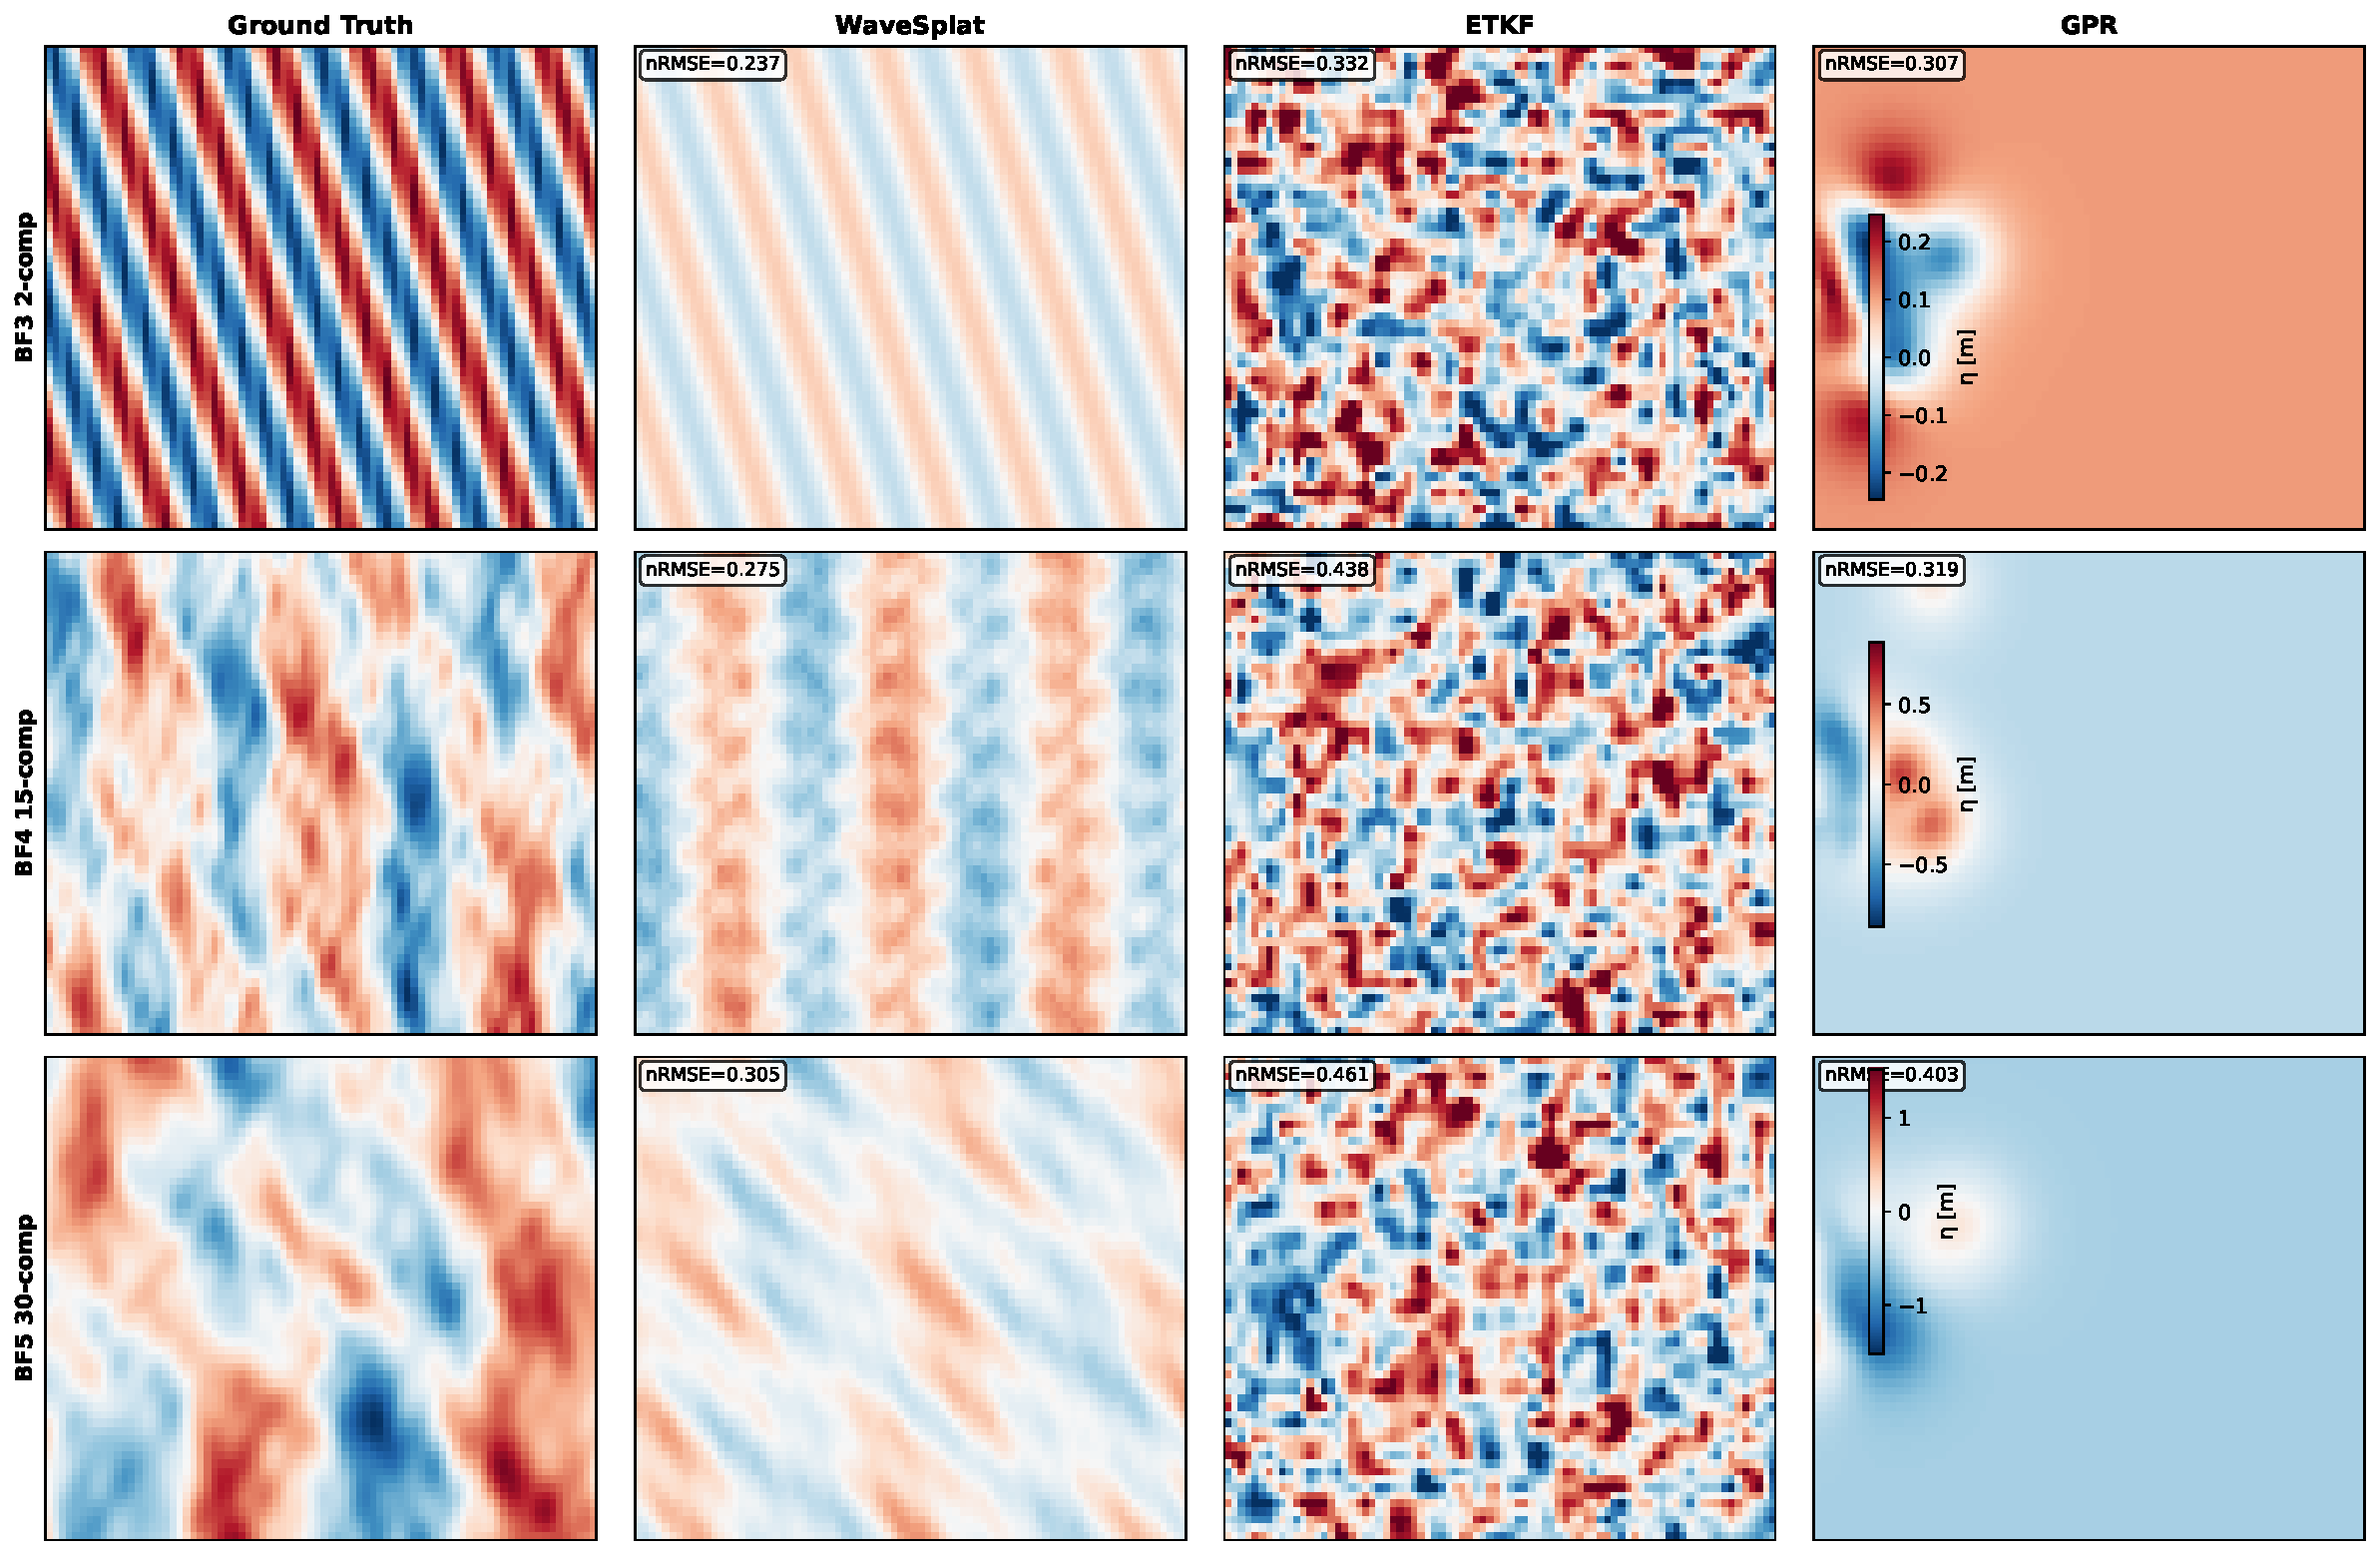
\includegraphics[width=\textwidth]{figures/fig8_qualitative.pdf}
\caption{Qualitative comparison on three episodes (rows: BF3 2-comp,
BF4 15-comp, BF5 30-comp). Columns: ground truth, WaveSplat, ETKF, GPR.
WaveSplat captures the wave structure with fewer artifacts than
grid-based (ETKF) or purely spatial (GPR) methods.}
\label{fig:qualitative}
\end{figure*}

% ============================================================================
\section{Discussion}
\label{sec:discussion}

\subsection{Advantages of grid-free representation}

The most striking result is the 8.5$\times$ advantage on 2-component
seas (nRMSE 0.052 vs.\ 0.444). For low-complexity wave fields, ETKF
wastes representational capacity on the full spatial grid when only two
spectral modes are present. WaveSplat's adaptive representation directly
captures the relevant modes with minimal parameters.

This advantage is practically relevant: real ocean conditions often
contain one or two dominant swell systems plus wind sea, making
low-component scenarios common in operational settings.
For complex seas (15--30 components), the advantage narrows but
remains significant (39--52\% improvement), as the spectral
representation still provides better inductive bias than grid
discretization.

\subsection{Convergence behavior}

Per-frame nRMSE curves show that WaveSplat converges rapidly after
initialization: BF3-2comp reaches nRMSE$<$0.05 within the first tracking
frame ($t$=11.6s). For complex seas (BF4--5), the nRMSE stabilizes
within the first 10\% of tracking frames, with minimal drift over the
remaining episode.  This fast convergence is enabled by the
dispersion-based phase prediction, which provides accurate warm starts
for each tracking frame.

\subsection{Role of the dispersion constraint}

The ablation reveals a nuanced role for the dispersion constraint.
On 30-second BF3 episodes, the unconstrained optimizer
achieves lower nRMSE (0.158 vs.\ 0.188) by exploiting the
additional frequency parameter to compensate for the $O(\epsilon^2)$
model mismatch with the Gerstner ground truth.

However, this result should not be interpreted as evidence against
the dispersion constraint.  The constraint serves as a \emph{structural
regularizer} that:
(1)~reduces the parameter count from $5N$ to $4N$, improving
robustness to overfitting on sparse observations;
(2)~enables physics-based phase prediction during tracking,
eliminating the need to re-estimate $\omega$ at each frame; and
(3)~ensures that the estimated wave field propagates according to
physical wave dynamics, which is essential for downstream
applications such as feedforward motion control that
require spatial evaluation at preview points.

The ablation was limited to BF3 conditions;
we expect the constraint to become more valuable at higher Beaufort
numbers where spectral crowding makes unconstrained frequency
estimation less reliable.

\subsection{Failure case: BF2 1-component}

WaveSplat's worst case (nRMSE=0.315) occurs on the simplest
episode: BF2, $H_s$=0.3~m, single component. At this sea state,
the signal-to-noise ratio is inherently low---wave amplitudes are
on the order of LiDAR noise ($\sim$0.02~m), making spectral
initialization unreliable. Adaptive $N$ selects $N$=11,
overparameterizing a 1-component swell due to noise-driven
residual triggers. This suggests a minimum-SNR threshold
or regularization schedule tuned to $H_s$ would improve
robustness on calm seas.

\subsection{Effect of observation model}

WaveSplat wins 10/10 under \emph{both} raydrop models.
Slope observations improve both methods---WaveSplat by 9.1\%
and ETKF by 16.2\%. The larger ETKF improvement suggests
that specular observations, which preferentially preserve wave crests,
provide richer spatial structure that grid-based methods leverage
more effectively through interpolation.
For adaptive~$N$, slope raydrop triggers the safety
rollback on low-complexity scenes (e.g., BF3-2comp: $N$=2$\to$15)
but enables more aggressive pruning on complex seas (BF4-15comp:
$N$=19$\to$10), indicating that stronger observations improve both
estimation and model selection.

\subsection{Practical deployment considerations}

WaveSplat's computational footprint (13.4~ms/frame, single CPU thread)
makes it suitable for deployment on standard shipboard computing
hardware.  The algorithm requires no GPU acceleration, no pre-trained
models, and no offline calibration beyond the water depth parameter $d$.
The spectral parameters are directly interpretable: a naval architect
can inspect the estimated wavenumber vector, amplitude, and frequency
of each component, enabling sanity checking against visual observation
and meteorological forecasts.

For integration with vessel control systems, the spectral representation
offers a key advantage: the estimated wave field can be evaluated at
\emph{any} spatial point via~\eqref{eq:forward} without interpolation.
This enables downstream applications such as wave-preview feedforward
control~\citep{park2026hydrofoil}, where the wave field must be
evaluated at spatial preview points ahead of the vessel.
Grid-based methods would require interpolation between grid points,
introducing additional error and latency.

\subsection{Comparison with higher-resolution ETKF}

A natural question is whether increasing the ETKF grid resolution
would close the performance gap.  Our implementation includes an
ETKF-fine variant (80$\times$60 grid, same ensemble size), which
achieves avg nRMSE of 0.421---only marginally better than the
standard 40$\times$30 grid (0.436), while running at 50--61~ms/frame.
This confirms that ETKF's performance is limited not by grid
resolution but by the ensemble-based estimation framework itself:
the finite ensemble size ($N_e = 50$) introduces sampling error
in the Kalman gain computation, and the linear observation operator
cannot fully exploit the nonlinear relationship between sparse
LiDAR geometry and the underlying wave field.

\subsection{Limitations and future work}

Several limitations should be acknowledged:

\begin{enumerate}
  \item \textbf{Simulation-only validation}: All results are obtained in
    simulation.  While the WaveSim environment models realistic LiDAR
    characteristics (beam divergence, raydrop, range-dependent noise),
    validation on real LiDAR data from wave tank experiments or
    sea trials is essential before operational deployment.
    The spectral representation and optimization framework are
    sensor-agnostic, but real LiDAR data may contain systematic
    biases (e.g., multi-path reflection, spray contamination) not
    captured by our noise model.
    We plan to validate using the wave tank facility at Seoul
    National University and subsequently on HD Hyundai's autonomous
    vessel testbed.
  \item \textbf{Linear forward model}: The $O(\epsilon^2)$ mismatch
    with nonlinear wave theories is small for the Beaufort~2--5 range
    but will become significant for steep waves approaching breaking
    ($\epsilon > 0.1$, typically BF6+).
    Extension to second-order Stokes theory, which captures bound
    harmonics as $O(\epsilon^2)$ corrections to the linear solution,
    is a natural next step that preserves the spectral parameterization
    while improving accuracy in steep seas.
  \item \textbf{Initialization resolution}: For $N_{\text{true}} \geq 30$
    components, the beamforming initialization cannot resolve all
    components due to spectral crowding in wavenumber space.
    Higher-resolution beamforming (denser wavenumber grid) or
    spatio-temporal 3D FFT (exploiting the full $(k_x, k_y, \omega)$
    volume) could address this, at the cost of increased initialization
    computation.
  \item \textbf{Current estimation}: The current implementation does
    not estimate ocean currents, which cause Doppler shifts in the
    observed wave field.  In the presence of currents, the apparent
    dispersion relation becomes
    $\omega = \sqrt{g|k|\tanh(|k|d)} + \mathbf{k} \cdot \mathbf{U}$,
    where $\mathbf{U}$ is the current velocity.
    Joint current-wave estimation by including $\mathbf{U}$ as a
    global parameter is a natural extension.
  \item \textbf{Baseline fairness}: The GPR comparison uses
    single-frame mode without temporal propagation.
    A sliding-window GPR with physics-based temporal kernel could
    provide a stronger baseline, and sparse GPR with inducing
    points could reduce the computational gap.
    However, incorporating the dispersion relation into a GPR
    kernel is non-trivial and remains an open research question.
  \item \textbf{Uncertainty quantification}: WaveSplat currently
    provides point estimates without uncertainty bounds.
    The optimizer's gradient information could be used to
    construct approximate confidence intervals via the Hessian,
    and ensemble techniques (running multiple initializations)
    could provide empirical uncertainty estimates.
\end{enumerate}

% ============================================================================
\section{Conclusion}
\label{sec:conclusion}

We presented WaveSplat, a grid-free spectral approach to
ocean wave field estimation from sparse shipboard LiDAR.
By representing waves as optimizable spectral components with
dispersion constraints and adaptive model complexity, WaveSplat achieves
51.5\% lower nRMSE than ETKF-grid while running 2.4$\times$ faster.
The advantage is statistically significant ($p < 0.001$, Wilcoxon
signed-rank test across 50 paired runs) and robust to both diffuse
and specular LiDAR observation models (20/20 wins).
The spectral representation also degrades gracefully under extreme
observation sparsity ($<$8\% degradation at 20\% observation density).

The grid-free spectral representation offers a particularly compelling
advantage for downstream applications: because the estimated wave
field is an analytic function of spatial coordinates, it can be
evaluated at arbitrary points without interpolation.
This property is directly exploited in a companion
paper~\citep{park2026hydrofoil}, where WaveSplat provides wave
preview information for feedforward motion control of hydrofoil vessels.

Future work includes validation on real LiDAR data from wave tank
experiments, extension to second-order wave models for steeper seas,
and joint estimation of ocean currents.
Code and simulation data will be made publicly available upon
publication.

% ============================================================================
\section*{CRediT authorship contribution statement}

\textbf{Saeyong Park}: Conceptualization, Methodology, Software,
Validation, Formal analysis, Investigation, Writing -- original draft,
Writing -- review \& editing, Visualization.

\section*{Declaration of competing interest}

The author declares no known competing financial interests or
personal relationships that could have appeared to influence
the work reported in this paper.

\section*{Data availability}

Code and simulation data will be made publicly available upon
acceptance.

\section*{Acknowledgments}

The author thanks the Avikus engineering team for discussions on
shipboard LiDAR integration and practical deployment considerations.

% ============================================================================
\bibliographystyle{elsarticle-num}
\bibliography{references}

\end{document}
